\documentclass[english,notitlepage, reprint]{revtex4-1}  % defines the basic parameters of the document
%For preview: skriv i terminal: latexmk -pdf -pvc filnavn



% if you want a single-column, remove reprint

% allows special characters (including æøå)
\usepackage[utf8]{inputenc}
%\usepackage[english]{babel}

%% note that you may need to download some of these packages manually, it depends on your setup.
%% I recommend downloading TeXMaker, because it includes a large library of the most common packages.

\usepackage{physics,amssymb}  % mathematical symbols (physics imports amsmath)
\usepackage{graphicx}         % include graphics such as plots
\usepackage{xcolor}           % set colors
\usepackage{hyperref}         % automagic cross-referencing (this is GODLIKE)
\usepackage{listings}         % display code
\usepackage{subfigure}        % imports a lot of cool and useful figure commands


\usepackage{float}
%\usepackage[section]{placeins}
\usepackage{algorithm}
\usepackage[noend]{algpseudocode}
\usepackage{subfigure}
% defines the color of hyperref objects
% Blending two colors:  blue!80!black  =  80% blue and 20% black
\hypersetup{ % this is just my personal choice, feel free to change things
    colorlinks,
    linkcolor={red!50!black},
    citecolor={blue!50!black},
    urlcolor={blue!80!black}}

\definecolor{codegreen}{rgb}{0,0.6,0}
\definecolor{codegray}{rgb}{0.5,0.5,0.5}
\definecolor{codepurple}{rgb}{0.58,0,0.82}
\definecolor{backcolour}{rgb}{0.95,0.95,0.92}

\lstdefinestyle{customc}{
	belowcaptionskip=1\baselineskip,
	breaklines=true,
	frame=L,
	xleftmargin=\parindent,
	language=C,
	showstringspaces=false,
	basicstyle=\footnotesize\ttfamily,
	keywordstyle=\bfseries\color{green!40!black},
	commentstyle=\itshape\color{purple!40!black},
	identifierstyle=\color{blue},
	stringstyle=\color{orange},
}

\lstdefinestyle{customasm}{
	belowcaptionskip=1\baselineskip,
	frame=L,
	xleftmargin=\parindent,
	language=[x86masm]Assembler,
	basicstyle=\footnotesize\ttfamily,
	commentstyle=\itshape\color{purple!40!black},
}

\lstset{escapechar=@,style=customc}

%% Defines the style of the programming listing
%% This is actually my personal template, go ahead and change stuff if you want



%% USEFUL LINKS:
%%
%%   UiO LaTeX guides:        https://www.mn.uio.no/ifi/tjenester/it/hjelp/latex/
%%   mathematics:             https://en.wikibooks.org/wiki/LaTeX/Mathematics

%%   PHYSICS !                https://mirror.hmc.edu/ctan/macros/latex/contrib/physics/physics.pdf

%%   the basics of Tikz:       https://en.wikibooks.org/wiki/LaTeX/PGF/Tikz
%%   all the colors!:          https://en.wikibooks.org/wiki/LaTeX/Colors
%%   how to draw tables:       https://en.wikibooks.org/wiki/LaTeX/Tables
%%   code listing styles:      https://en.wikibooks.org/wiki/LaTeX/Source_Code_Listings
%%   \includegraphics          https://en.wikibooks.org/wiki/LaTeX/Importing_Graphics
%%   learn more about figures  https://en.wikibooks.org/wiki/LaTeX/Floats,_Figures_and_Captions
%%   automagic bibliography:   https://en.wikibooks.org/wiki/LaTeX/Bibliography_Management  (this one is kinda difficult the first time)
%%   REVTeX Guide:             http://www.physics.csbsju.edu/370/papers/Journal_Style_Manuals/auguide4-1.pdf
%%
%%   (this document is of class "revtex4-1", the RVTeX Guide explains how the class works)


%% CREATING THE .pdf FILE USING LINUX IN THE TERMINAL
%%
%% [terminal]$ pdflatex template.tex
%%
%% Run the command twice, always.
%% If you want to use \footnote, you need to run these commands (IN THIS SPECIFIC ORDER)
%%
%% [terminal]$ pdflatex template.tex
%% [terminal]$ bibtex template
%% [terminal]$ pdflatex template.tex
%% [terminal]$ pdflatex template.tex
%%
%% Don't ask me why, I don't know.

\begin{document}
\title{Home exam 1 - IN3200}      % self-explanatory
\author{Candidate nr: 15129}          % self-explanatory
\date{\today}                             % self-explanatory
\noaffiliation                            % ignore this
                                          % marks the end of the abstracthttps://github.com/reneaas/fys2160.git

\maketitle
\section{Introduction}
In this report we look into the main algorithmic aspects of the code implementations and present time measurements of the serial and parallelized codes. The important computer and software specifications for the benchmarks in the report is shown in table \ref{tab:specs}.
\begin{table}[H]
	\centering
	\begin{tabular}{c@{\hspace{2cm}}c}
		\hline
		GCC compiler & 9.3.1 \\
		OS & Clear Linux OS vers. 32660\\
		CPU & Intel i7-8565U\\
		\hline
	\end{tabular}\caption{The table shows the most important software and hardware specifications to reproduce the results presented in this report.}\label{tab:specs}
\end{table}

\section{Background}

\subsection*{Webgraphs}
Webgraphs describe hyperlinks between to webpages $i$ and $j$. Each webpage is represented by a node and the hyperlink between them is known as an edge. In this report I'll define $N$ as the number of nodes and $N_\text{links}$ as the number of edges in a \textit{directed }webgraph. By directed, we mean that the hyperlink $j\to i$ is distinct from $i \to j$.

\subsection*{Hyperlink matrix representation of webgraphs}
Webgraphs can be represented by what is called a hyperlink matrix $A$. An element $A_{ij} = 1$ if there exists a hyperlink $j \to i$. If no such link exists, $A_{ij} = 0$. In the implementation described in this report, we allow no self-links $i \to i$ such that $A_{ii} = 0$ for all $i$.

\subsection*{Compressed row storage (CRS) of the hyperlink matrix}
For large webgraphs, it's expected that the hyperlink matrix will mainly consist of zeros. Since the storage in the matrix format scales with $N^2$, storing the data becomes a bottleneck. The CRS format is based on two different arrays. There's the \textit{row pointer} which stores information about how many row elements the webgraph has. Let $r$ denote the row pointer array. The following equation shows the general form of this array.
\begin{equation}\label{eq:row_pointer}
	r = (0, r_0, r_0 + r_1,..., r_0 + r_1 + \cdots + r_{N-1}),
\end{equation}
where $r_i$ is the number of row elements of row $i$. The row pointer thus has length $N+1$. To extract how many row elements there are on row $i$, we take the difference $r_{i}-r_{i-1}$. The second array is called a \textit{column index} array and is of length $N_\text{links}$ and stores the column indices for each row.

\subsection*{Mutual web linkages and number of involvements}
\textit{Mutual web linkages} is defined as the number of times to outbound nodes $i$ and $j$ are directly linked to a inbound node $k$, with $i \neq j \neq k$. That is, it's a count of how many times there exists a hyperlink $i \to k$ and $j\to k$ simultaneously. The \textit{number of involvements} a given node has is defined as the number of times a given node is involved as an outbound node. That is how many times a node $i$ is involved in $i \to k$ with $j\to k$.

\section{Implementation}
\subsection*{Reading the Webgraph from file}
\subsubsection{Hyperlink matrix storage}
To extract the data to store in a hyperlink matrix is straight forward. The following code snippet shows how I did it.
\begin{lstlisting}[style=customc]
int FromNodeId, ToNodeId;
for (int k = 0; k < N_links; k++){
  fscanf(fp, "%d %d", &FromNodeId, &ToNodeId);
  (*table2D)[ToNodeId][FromNodeId] = (char) 1;
}
\end{lstlisting}

\subsubsection{CRS storage}
To extract the data from the file into CRS storage, we must first sort the arrays. I chose to sort this using the \textit{shellsort} algorithm with $\text{gap} = N/2$. The following code snippet shows the implementation.

\begin{lstlisting}[style=customc]
int tmp1, tmp2, i, j, gap;
for (gap = *N_links/2; gap > 0; gap /= 2){
  for (i = gap; i < *N_links; i++){
  tmp1 = row_elems[i];
  tmp2 = (*col_idx)[i];
  for (j = i; j >= gap && row_elems[j-gap] > tmp1; j -= gap){
    row_elems[j] = row_elems[j-gap];
    (*col_idx)[j] = (*col_idx)[j-gap];
  }
  row_elems[j] = tmp1;
  (*col_idx)[j] = tmp2;
  }
}
\end{lstlisting}
Here, row\_elems is just there to temporarily store row node ids. The row pointer is simply made using an array counting how many elements each row has consistent with eq. \eqref{eq:row_pointer}. The following code demonstrates this.
\begin{lstlisting}[style=customc]
*row_ptr = (int*)calloc(*N+1, sizeof(int*));
int count = 0;
for (int i = 0; i < *N; i++){
  count += row_count[i];
  (*row_ptr)[i+1] = count;
}
\end{lstlisting}

\subsection*{Counting mutual web links}
\subsubsection{Counting mutual web links with the hyperlink matrix}
To count the number of web links that each node is an outbound participant is in principle a simple matter when we use the hyperlink matrix representation. It is simply to check when $A_{ij} = A_{ik} = 1$ with $i\neq j \neq k$. However, to make the code implementation efficient, it's important to do this economically. The algorithm goes as follows: For a given node $i$, we check every $j$ and only if $A_{ij} = 1$ should we count the mutual linkages and number of involvements. One way to do this is to insert an if test and check if $A_{ik} = 1$ and add $1$ to both variables. However, since $A_{ik}$ is either $0$ or $1$, we might as well just add the matrix element itself and avoid the if-test entirely. The following code demonstrates how this can be implemented. It also counts the total number of web linkages
which is just the total number of times mutual web links occur.

\begin{lstlisting}[style=customc]
int counter;
for (i = 0; i < N; i++){
  for (j = 0; j < N; j++){
    counter = 0;
    if (table2D[i][j] == 1){
      for (k = j+1; k < N; k++){
        counter += table2D[i][k];
        num_involvements[k] += table2D[i][k];
      }
      num_involvements[j] += counter;
      total_mutual_web_linkages += counter;
    }
  }
}
\end{lstlisting}

\subsubsection{Counting mutual web links with the CRS format}
To count the total number of web links in this format, we can reduce the number of floating point operations by computing the sum analytically. To find the contribution a given row $i$ has to the total number of web linkages, let's first define $m_i$ to be the number of elements on row $i$ such that $m_i = r_i - r_{i-1}$. Then
\begin{equation}
    S = \sum_{k = 0}^{m_i-1} k = \frac{m_i(m_i-1)}{2},
\end{equation}
where the standard formula for the sum of the $m_i-1$ first integers were used. The following code snippet shows the implementation.

\begin{lstlisting}[style=customc]
for (int i = 0; i < N; i++){
  tmp = row_ptr[i];
  row_elems = row_ptr[i+1]-tmp;
  for (int j = 0; j < row_elems; j++){
    num_involvements[col_idx[j+tmp]] += row_elems-1;
  }
  total_mutual_web_linkages += (row_elems)*(row_elems-1);
}
total_mutual_web_linkages *= 0.5;
\end{lstlisting}
As can be seen from the code, a tmp variable is defined to avoid loading row\_ptr[$i$] in $j$-dependent loop. In addition we use the sum formula instead of computing the actual sum for each $i$ manually.

\subsection*{Finding top webpages}
First of all, by top webpages we mean the webpages or nodes that are most involved as an outbound node in mutual linkages. To find the $n$ top webpages in a webgraph, I've used shellsort again, but this time sorting in descending order. For small $n$ this isn't the wisest choice since the algorithm is only dependent on how many nodes there are. However, for larger $n$'s it's an efficient choice. The code implementation is as follows.
\begin{lstlisting}[style=customc]
int gap, i, j, tmp1, tmp2;
  for (gap = num_webpages/2; gap > 0; gap /= 2){
  for (i = gap; i < num_webpages; i++){
    tmp1 = num_involvements[i];
    tmp2 = webpage_number[i];
    for (j = i; j >= gap && num_involvements[j-gap] < tmp1; j -= gap){
      num_involvements[j] = num_involvements[j-gap];
      webpage_number[j] = webpage_number[j-gap];
    }
    num_involvements[j] = tmp1;
    webpage_number[j] = tmp2;
  }
}
\end{lstlisting}

\subsection*{Parallelization of count\_mutual\_links1}
To parallelize this function is straight forward by applying the following OpenMP directive on the outer loop
\begin{lstlisting}[style=customc]
#pragma omp parallel for private(i, j, k) reduction(+: total_mutual_web_linkages, num_involvements[:N])
\end{lstlisting}
This is because we need to make the indices $i$, $j$ and $k$ private to each thread. To handle the possibility of race conditions when reading and updating the total\_mutual\_web\_linkages
and elements in num\_involvements, we must also use the reduction clause.

\subsection*{Parallelization of count\_mutual\_links2}
This function is also readily parallelizable, but also here we must avoid race conditions. Here, however, we can use the \#pragma omp atomic directive instead (simply because it provided more speedup than using the reduction clause on the array elements). The following code shows the parallelized version.
\begin{lstlisting}[style=customc]
int tmp, row_elems;
#pragma omp parallel for private(tmp, row_elems) reduction(+:total_mutual_web_linkages)
for (int i = 0; i < N; i++){
  tmp = row_ptr[i];
  row_elems = row_ptr[i+1] - tmp;
  for (int j = 0; j < row_elems; j++){
    //Insert atomic to avoid race conditions when updating num_involvements.
    #pragma omp atomic
    num_involvements[col_idx[j+tmp]] += row_elems-1;
  }
  total_mutual_web_linkages += (row_elems)*(row_elems-1);
}
\end{lstlisting}


\section{Results}

\subsection*{Timing of serial codes}
The measured time of the serial implementations of the various functions are shown in table \ref{tab:serial_codes}.
\begin{table}[h!]
	\centering
	\begin{tabular}{c@{\hspace{2cm}}c}
		\hline
		Function name & Time in seconds \\
		\hline
		read\_graph\_from\_file1 & $0.179096$\\
		count\_mutual\_links1 & $1.799104$\\
		read\_graph\_from\_file2 & $0.356536$\\
		count\_mutual\_links2 & $0.001885$\\
		top\_n\_webpages & $0.019348$\\
		\hline
	\end{tabular}\caption{The table shows the measured time using clock() from the Ctime-library. read\_graph\_from\_file1 and count\_mutual\_links1 was applied to a web-graph containing $N = 5000$ nodes and $N_\text{links} = 146823$ edges as found in the file test\_webpages.txt. The data in this file was extracted from web-NotreDame.txt.  read\_graph\_from\_file2 and count\_mutual\_links2 was applied directly to the web-graph contained in web-NotreDame.txt. This file contained $N = 325729$ nodes and $N_\text{links} = 1479143$ edges.}\label{tab:serial_codes}
\end{table}

\subsection*{Parallelized version of count\_mutual\_links1}
Using OpenMP to parallelize count\_mutual\_links1 gave the time measurements shown in figure \ref{fig:count_mutual_links1_parallel}.
\begin{figure}[H]
    \centering
    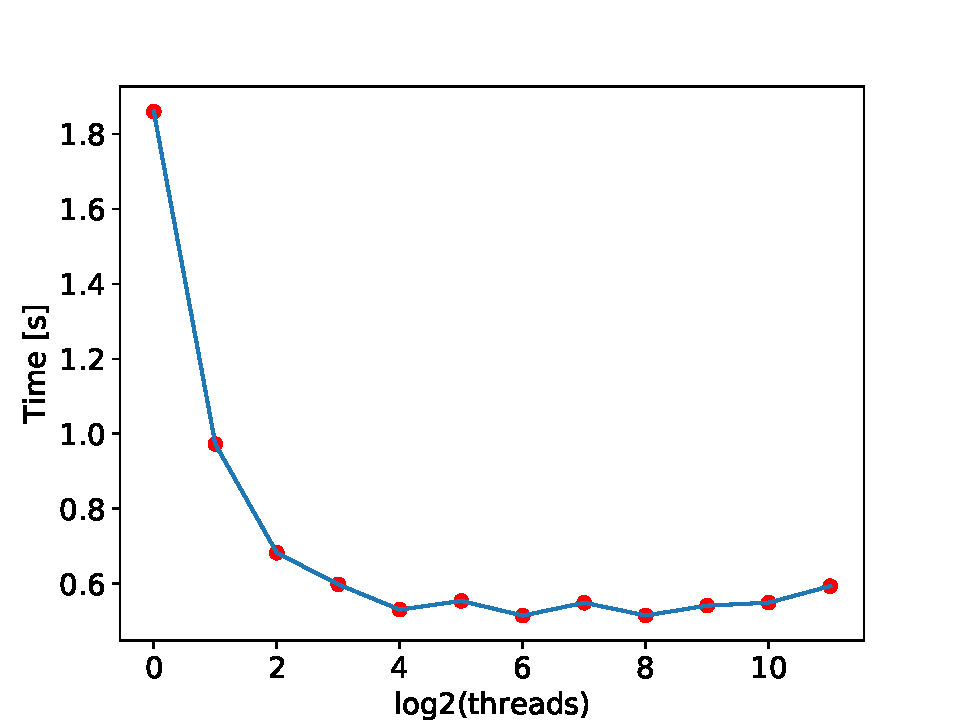
\includegraphics[scale = 0.5]{count_mutual_links1_parallel.pdf}
    \caption{The figure shows the time used  in seconds by count\_mutual\_links1 on a webgraph consisting of $N = 50000$ nodes and $N_\text{links} = 146823$ edges. The webgraph was extracted from web-NotreDame.txt. The red points show the actual measured datapoints.}\label{fig:count_mutual_links1_parallel}
\end{figure}
The speedup relative to one thread is shown in figure \ref{fig:count_mutual_links1_speedup}.
\begin{figure}[H]
    \centering
    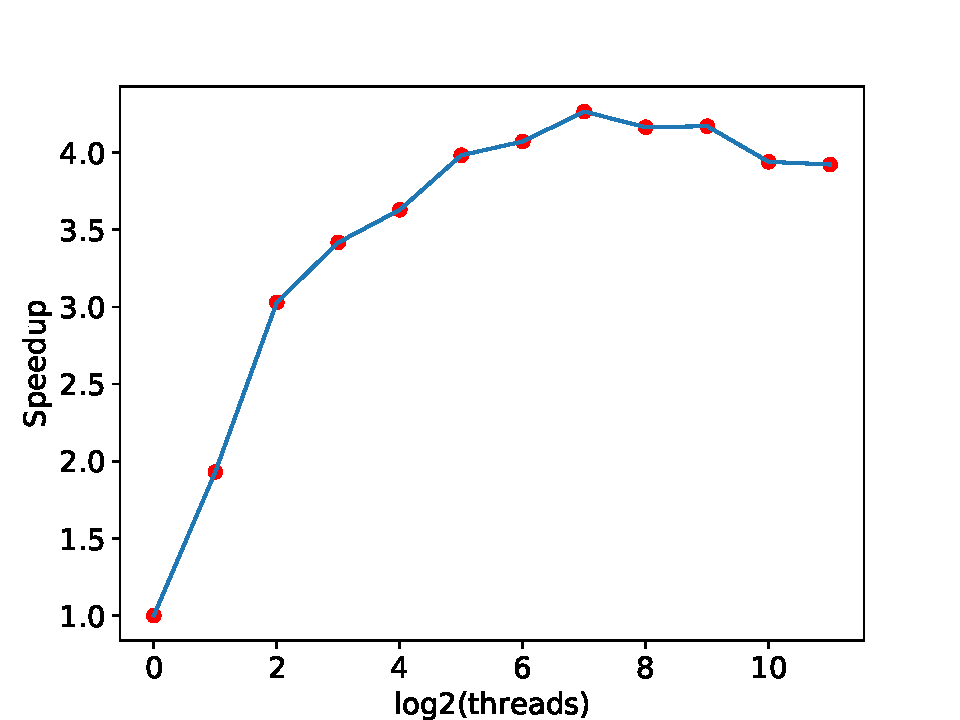
\includegraphics[scale = 0.5]{count_mutual_links1_speedup.pdf}
    \caption{The figure shows speedup relative to a single thread by count\_mutual\_links1 on a webgraph consisting of $N = 50000$ nodes and $N_\text{links} = 146823$ edges. The webgraph was extracted from web-NotreDame.txt. The red points show the actual measured datapoints.}\label{fig:count_mutual_links1_speedup}
\end{figure}

\subsection*{Parallelized version of count\_mutual\_links2}
Using OpenMP to parallelize count\_mutual\_links2 and measuring the time used by the function for different number of threads yielded the results shown in figure \ref{fig:count_mutual_links2_parallel}.
\begin{figure}[H]
    \centering
    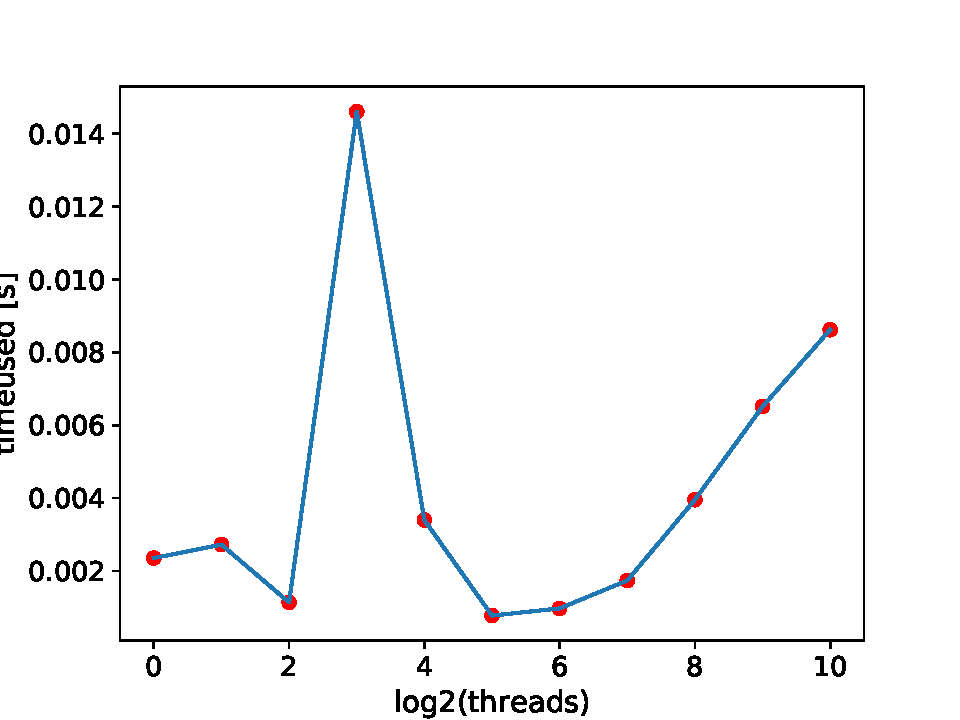
\includegraphics[scale = 0.5]{count_mutual_links2_parallel.pdf}
    \caption{The figure shows the time used  in seconds by count\_mutual\_links2 on a webgraph consisting of $N = 325729$ nodes and $N_\text{links} = 1479143$ edges. The webgraph is found in the file web-NotreDame.txt}\label{fig:count_mutual_links2_parallel}
\end{figure}
The speedup relative to a single thread is shown in figure \ref{fig:count_mutual_links2_speedup}.
\begin{figure}[H]
    \centering
    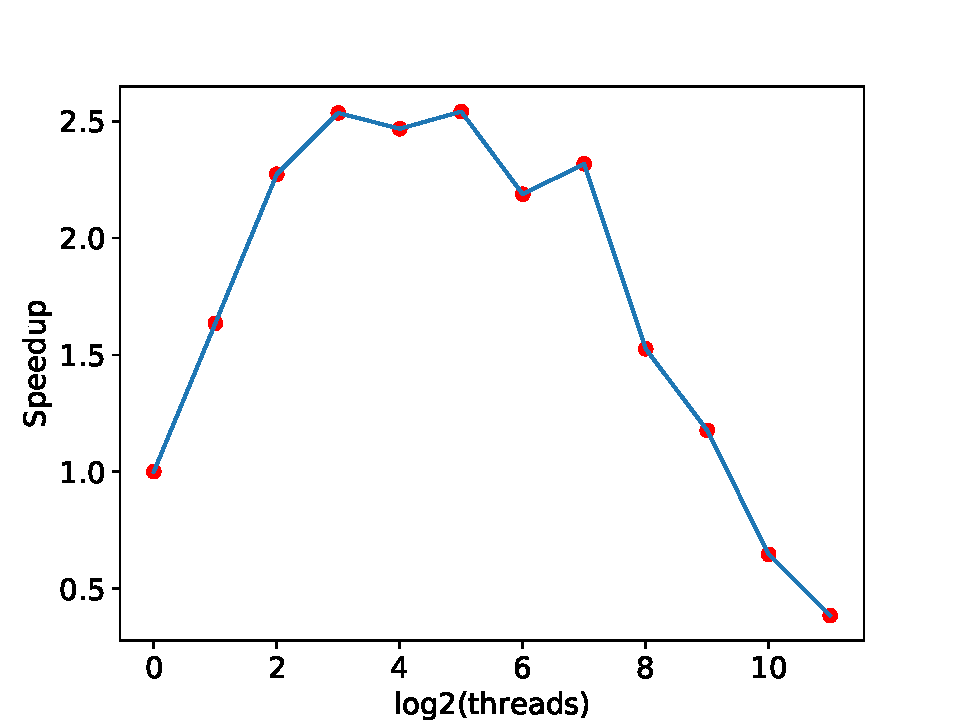
\includegraphics[scale = 0.5]{count_mutual_links2_speedup.pdf}
    \caption{The figure shows speedup relative to a single thread by count\_mutual\_links1 on a webgraph consisting of $N = 325729$ nodes and $N_\text{links} = 1479143$ edges. The webgraph is from the file web-NotreDame.txt. The red points show the actual measured datapoints.}\label{fig:count_mutual_links2_speedup}
\end{figure}

\section{Concluding Remarks}



\end{document}
